% Created 2017-06-20 Tue 04:18
% Intended LaTeX compiler: pdflatex
\documentclass[11pt]{article}
\usepackage[utf8]{inputenc}
\usepackage[T1]{fontenc}
\usepackage{graphicx}
\usepackage{grffile}
\usepackage{longtable}
\usepackage{wrapfig}
\usepackage{rotating}
\usepackage[normalem]{ulem}
\usepackage{amsmath}
\usepackage{textcomp}
\usepackage{amssymb}
\usepackage{capt-of}
\usepackage{hyperref}
\author{Francesco Ferraro}
\date{Porto Alegre 17/06/2017}
\title{Defesa Prefeitura Porto Alegre}
\hypersetup{
 pdfauthor={Francesco Ferraro},
 pdftitle={Defesa Prefeitura Porto Alegre},
 pdfkeywords={},
 pdfsubject={},
 pdfcreator={Emacs 25.2.1 (Org mode 9.0.7)},
 pdflang={'pt_Br'}}
\begin{document}

\maketitle
Venho por meio desta, apresentar a defesa referente aos seguintes
autos de infração, que chagaram até meu conhecimento em data
diferente e de modos diferentes.

\begin{center}
\begin{tabular}{rll}
Número & Endereço & Data\\
\hline
1007706 & Av. Carlos Barbosa 998 & 19/04\\
1007704 & Av. Carlos Barbosa 1000 & 19/04\\
1007704 & Av. Carlos Barbosa 1002/Sala2 & 19/04\\
1007704 & Av. Carlos Barbosa 1004 & 19/04\\
1007704 & Av. Carlos Barbosa 1006 & 19/04\\
\end{tabular}
\end{center}


\section{Defesa}
\label{sec:org38acf5a}

Meu nome é \textbf{Francesco Ferraro}, CPF \textbf{135.311.900-91}, proprietário de
\textbf{toda} a edificação localizada na esquina da Av. Carlos Barbosa com a
Rua Oscar Schineider. E esse é o primeiro argumento com que baseio a
minha defesa. O prédio possui carta de habitação e planta, anexados
nesse protocolo, aprovadas pela Prefeitura de Porto Alegre que
subdividem a edificação em quatro lojas e dois
apartamentos. Entretanto, o proprietário de todas as unidades são a
mesma pessoa, no caso, eu.  Por isso, antes de apresentar minha
defesa, peço a unificação das infrações recebidas em uma única
multa.  Foram aplicadas multa até nos aparatamentos que ficam
localizados no segunda andar. Pelo princípio do "non bis in idem",
garantido pela nossa constituição, que diz que ninguém pode ser
condenado pelo mesmo infração duas vezes, peço mais uma vez que
todas essas infrações sejas analisadas e conjugadas.
\newpage

Segue anexo também cópia da planta aprovada por essa mesma prefeitura
aprovando o rebaixo no meio. É um documento válido que comprova a
regularidade do meio fio. Vale ressaltar também que o local se
encontra em condições iguais às representadas em planta. Abaixo segue
foto da planta em que consta o rebaixo do meio fio aprovado.


\begin{figure}[htbp]
\centering
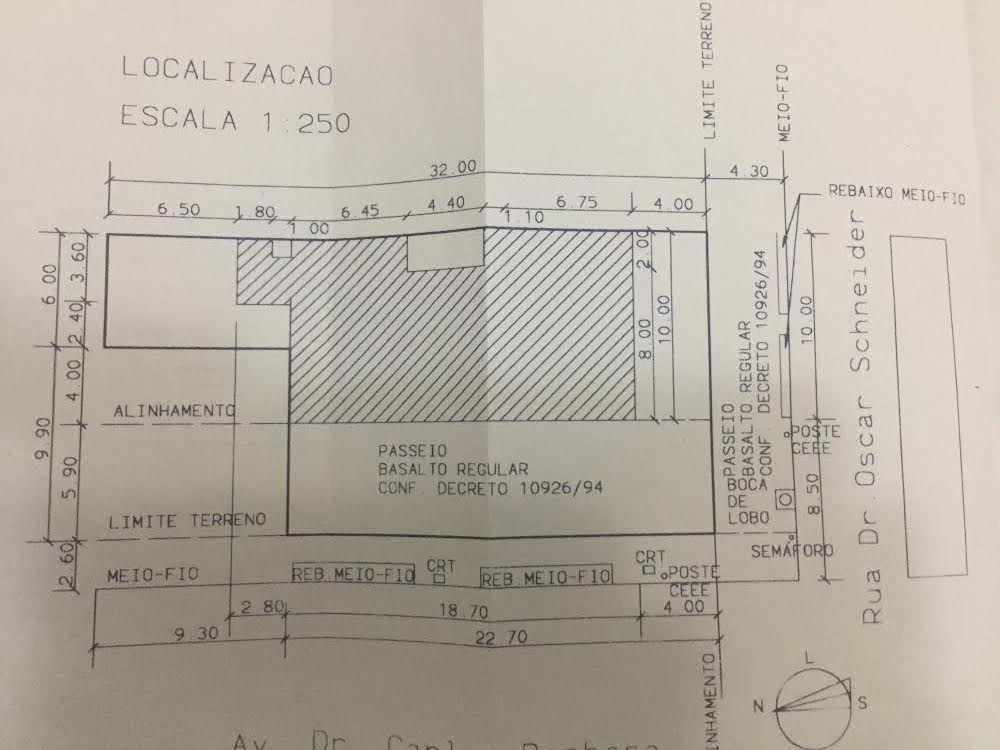
\includegraphics[width=.9\linewidth]{unnamed.jpg}
\caption{\label{fig:orga569bc6}
Planta Aprovada pela PMPA}
\end{figure}
\end{document}
